\documentclass[12pt]{article}
 
\usepackage[margin=1in]{geometry} 
\usepackage{amsmath,amsthm,amssymb,bm}
\usepackage{graphicx}
\usepackage[ruled]{algorithm2e} % Algorithms 
\usepackage[caption = false]{subfig}
 
\begin{document}
  
\title{Task 3. Reinforcement Learning}
\author{Garoe Dorta-Perez\\
CM50245: Computer Animation and Games II}
 
\maketitle
 
\section{Introduction}

\section{A* path finding}

The A* algorithm can find paths optimally in a graph based on a heuristic.
It works under the assumption that the distance heuristic will never overestimate the cost of the path and the path cost will not decrease as we travel through it.
In a maze world, where the movement possibilities are north, south, east and west, with fixed positive costs.
Using a Manhattan distance for the actual path cost and a euclidean distance to compute the heuristic will fit the assumptions.

In Algorithm \ref{alg:A_start} an overview of a general implementation of the A* in pseudocode is given.
As stated in the previous paragraph, in our case, graph.cost() and heuristic() returns respectively, the Manhattan and the euclidean distance between two nodes. An example output with a small labyrinth where a path is successfully found is shown in Figure \ref{fig:A_start}.

\begin{algorithm}[htbp!] \label{alg:A_start}
	\caption{A*}
	\KwData{$goal$ goal position, $start$ start position, $graph$ graph with the tiles in the map.}
	\KwResult{$path$ path from $start$ to $goal$, $cost$ total cost of the path.}
	
	frontier = PriorityQueue()\;
	frontier.put(start, 0)\;
	came\_from = \{\}\;
	cost\_so\_far = \{\}\;
	came\_from[start] = None\;
	cost\_so\_far[start] = 0\;

	\While{not frontier.empty()}{
		current = frontier.get()\;

		\If{current == goal}{
		  break\;
		}
		\For{next in graph.neighbors(current)}{
		  new\_cost = cost\_so\_far[current] + graph.cost(current, next)\;
		  \If{next not in cost\_so\_far or \text{new}\_cost \textless cost\_so\_far[next]}{
			 cost\_so\_far[next] = new\_cost\;
			 priority = new\_cost + heuristic(goal, next)\;
			 frontier.put(next, priority)\;
			 came\_from[next] = current\;
			 }
		}
	}
	$path$ = getPath(came\_from)\;
	$goal$ = cost\_so\_far[current]\;
\end{algorithm}

\begin{figure}[htbp!]
\centering
\begin{minipage}[t]{0.3\linewidth}
	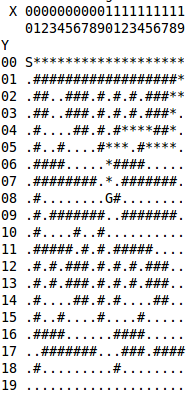
\includegraphics[scale=0.6]{images/a_star_res1}
	\caption{Path finding example, $S$ is the start position, $G$ is the goal position, $*$ are the path points, $.$ are empty spaces and \# are walls.}
	\label{fig:A_start}
\end{minipage}
\quad
\begin{minipage}[t]{0.3\linewidth}
	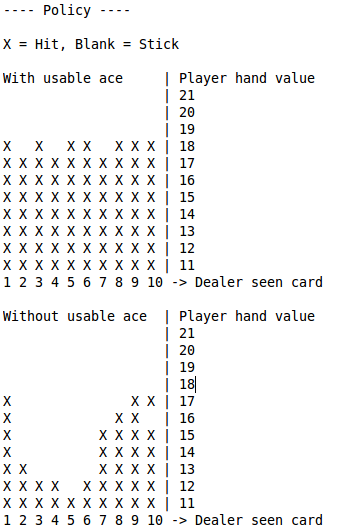
\includegraphics[scale=0.35]{images/blackjack_0_2_Q}
	\caption{Blackjack policy example, with 20\% exploration rate after 100000 games.}
	\label{fig:blackjack_0_2_Q}
\end{minipage}
\quad
\begin{minipage}[t]{0.3\linewidth}
	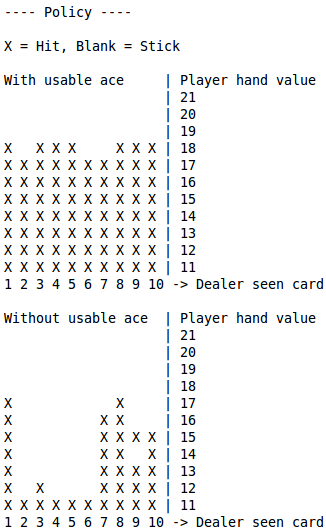
\includegraphics[scale=0.35]{images/blackjack_0_4_Q}
	\caption{Blackjack policy example, with 40\% exploration rate after 100000 games.}
	\label{fig:blackjack_0_4_Q}
\end{minipage}
\end{figure}

\section{Q learning in noughts and crosses}

\begin{figure}[htbp!]
\centering
	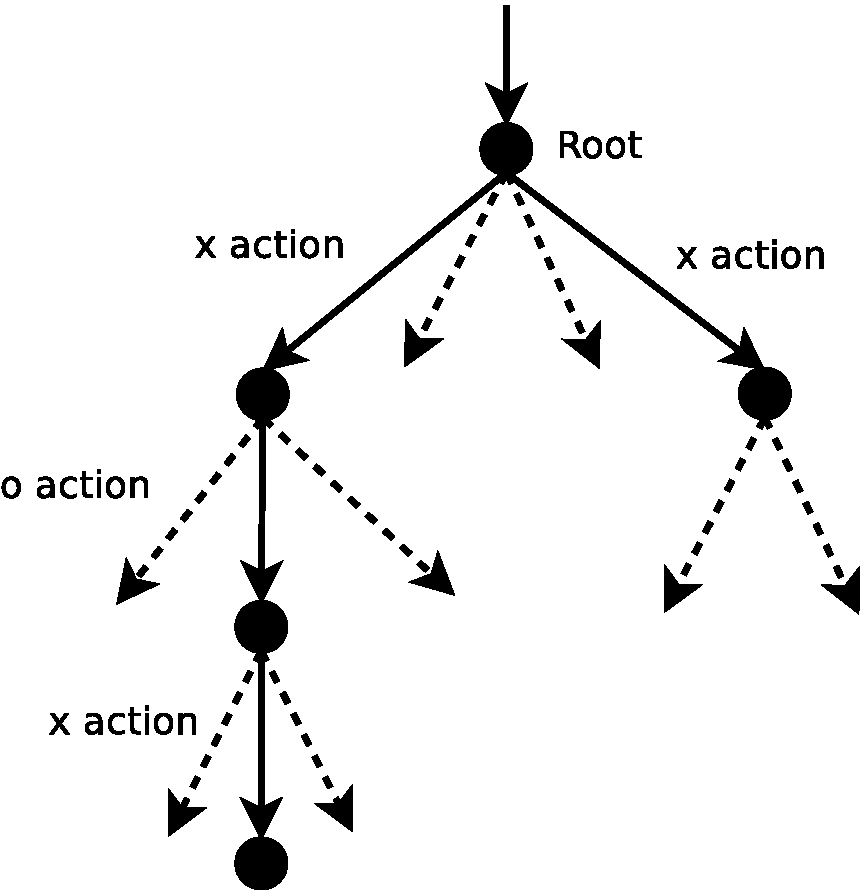
\includegraphics[scale=0.4]{images/ttt_tree}
	\caption{Path finding example, $S$ is the start position, $G$ is the goal position, $*$ are the path points, $.$ are empty spaces and \# are walls.}
	\label{fig:A_start}
\end{figure}

\section{Q learning in BlackJack}

\section{Results and conclusions}

%\bibliographystyle{plain}
%\bibliography{t2_meshAnim}

\end{document}




\end{document}

